\documentclass[border=10mm]{standalone}
% \usepackage[a4paper,top=2cm,bottom=2cm,left=2cm,right=2cm]{geometry}
\usepackage[margin=1in]{geometry}
\usepackage{graphicx}
\usepackage{bm}
\usepackage{pgfplots}
\usepackage{tikz}
\usetikzlibrary{calc}
\def\MarkRightAngle[size=#1](#2,#3,#4){
  \draw[] ($(#3)!#1!(#2)$) -- ($($(#3)!#1!(#2)$)!#1!90:(#2)$) -- ($(#3)!#1!(#4)$)
}

\usetikzlibrary{patterns}
\usetikzlibrary{angles,quotes}
\usepackage{parskip}
\usetikzlibrary{intersections, pgfplots.fillbetween}
\usepackage{amsmath}
\usepackage{multicol}
\usepackage{enumitem}
\usepackage{multirow}


\begin{document}

\tikzset{every picture/.style={line width=0.75pt}} %line width to 0.75pt        

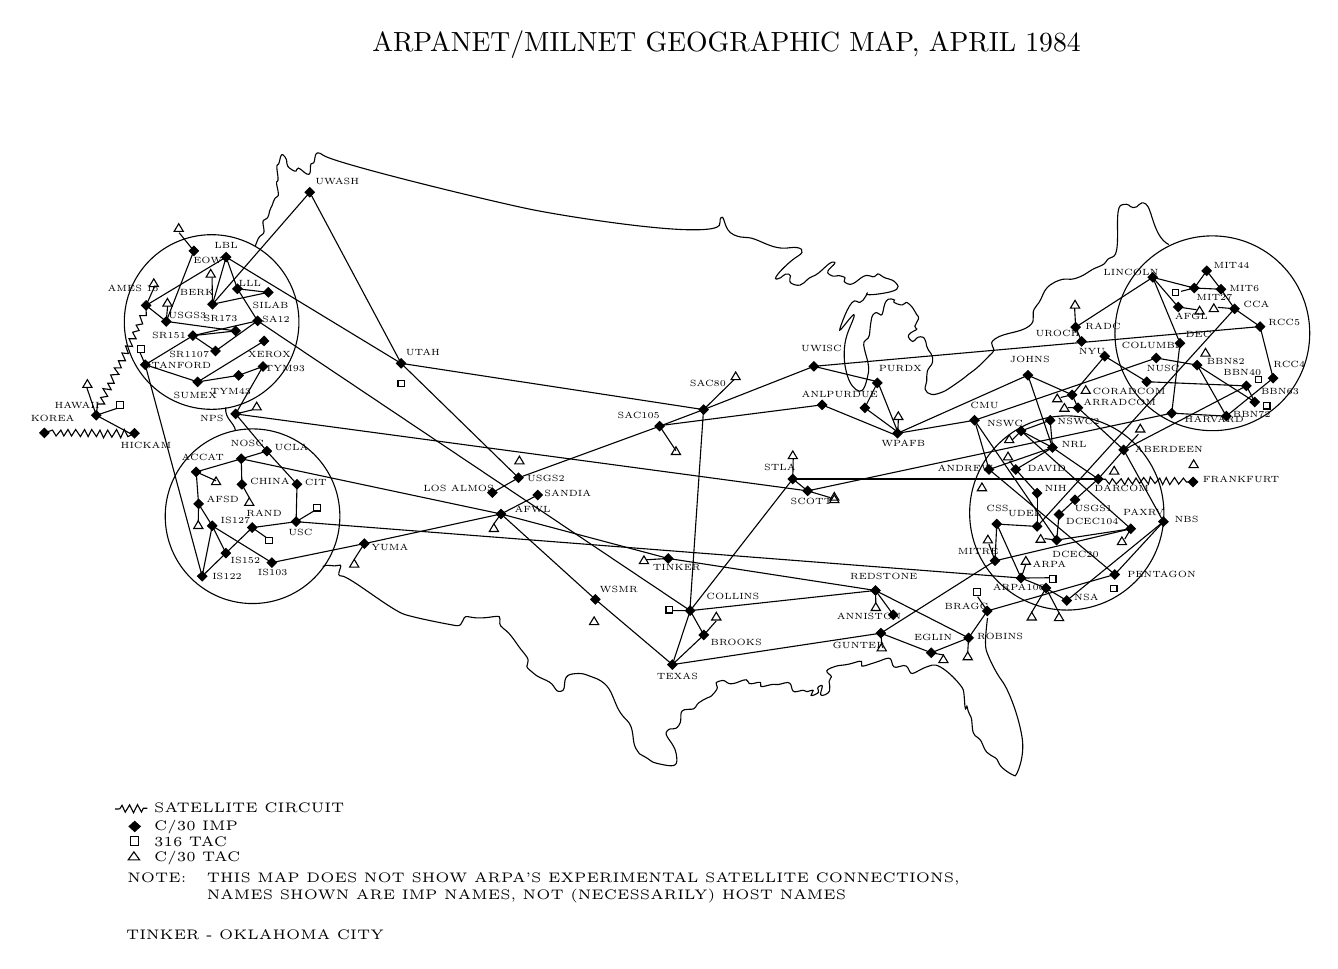
\begin{tikzpicture}[x=0.75pt,y=0.75pt,yscale=-1,xscale=1]
%uncomment if require: \path (0,528); %set diagram left start at 0, and has height of 528



%Curve Line of Map (top)  
\draw    (121.56,120.5) .. controls (122.78,117.67) and (122.8,116.17) .. (125,115) .. controls (127.2,113.83) and (123.67,108.33) .. (126.11,107.89) .. controls (128.56,107.44) and (127.89,103.89) .. (129,102.33) .. controls (130.11,100.78) and (130.33,97.22) .. (132.11,96.78) .. controls (133.89,96.33) and (130.78,89.67) .. (132.11,89.44) .. controls (133.44,89.22) and (131,81.67) .. (132.33,81.44) .. controls (133.67,81.22) and (133.22,74.11) .. (135.67,77.44) .. controls (138.11,80.78) and (134.93,81.13) .. (139.22,83.89) .. controls (143.51,86.64) and (139.44,80.11) .. (144.78,84.78) .. controls (150.11,89.44) and (146.78,80.33) .. (149,80.78) .. controls (151.22,81.22) and (148.78,72.78) .. (154.11,76.78) .. controls (159.44,80.78) and (238.56,99.89) .. (255.67,103.22) .. controls (272.78,106.56) and (311.67,112.56) .. (331.22,112.78) .. controls (350.78,113) and (343.89,108.78) .. (345.89,107) .. controls (347.89,105.22) and (346.88,112.95) .. (352.11,115.22) .. controls (357.34,117.49) and (357.92,115.38) .. (363.67,117.89) .. controls (369.41,120.4) and (373.44,122.33) .. (379,121.44) .. controls (384.56,120.56) and (387.22,123) .. (383,125.44) .. controls (378.78,127.89) and (369.67,137) .. (372.78,136.56) .. controls (375.89,136.11) and (375.89,133.44) .. (378.56,134.11) .. controls (381.22,134.78) and (376.41,137.76) .. (381.22,139.22) .. controls (386.04,140.68) and (386.11,136.56) .. (390.11,135.22) .. controls (394.11,133.89) and (397.89,127.67) .. (400.33,128.33) .. controls (402.78,129) and (394.81,132.41) .. (398.11,134.33) .. controls (401.41,136.26) and (400.78,134.11) .. (404.33,135.22) .. controls (407.89,136.33) and (402.95,136.92) .. (406.78,138.78) .. controls (410.61,140.63) and (413.54,133.27) .. (417.67,135) .. controls (421.8,136.73) and (419.9,132.38) .. (423,134.78) .. controls (426.1,137.17) and (427.58,135.74) .. (430.11,138.33) .. controls (432.64,140.93) and (431.44,142.33) .. (422.11,143.67) .. controls (412.78,145) and (417.22,142.56) .. (416.33,143.67) .. controls (415.44,144.78) and (413.89,149.22) .. (411.22,147.22) .. controls (408.56,145.22) and (404.56,156.33) .. (403.22,160.33) .. controls (401.89,164.33) and (410.11,151.67) .. (410.11,153.89) .. controls (410.11,156.11) and (406.56,161.44) .. (405.67,167.44) .. controls (404.78,173.44) and (405.44,178.56) .. (406.78,183) .. controls (408.11,187.44) and (410.33,189.89) .. (412.56,190.56) .. controls (414.78,191.22) and (416.11,186.11) .. (417,181.22) .. controls (417.89,176.33) and (412.78,167.44) .. (415.44,166.11) .. controls (418.11,164.78) and (417.36,162.28) .. (417.89,159) .. controls (418.42,155.72) and (418.4,153.96) .. (419.89,153) .. controls (421.38,152.04) and (421.44,153.44) .. (423,153.89) .. controls (424.56,154.33) and (423.68,145.26) .. (427.89,146.11) .. controls (432.1,146.97) and (426.41,146.84) .. (431,148.56) .. controls (435.59,150.27) and (433.67,146.11) .. (436.56,148.56) .. controls (439.44,151) and (439.67,153.67) .. (441,154.56) .. controls (442.33,155.44) and (437.67,159.67) .. (439.89,160.33) .. controls (442.11,161) and (433.89,162.33) .. (436.78,165.44) .. controls (439.67,168.56) and (438.7,164.31) .. (442.11,164.33) .. controls (445.53,164.36) and (444.11,168.78) .. (445.89,170.78) .. controls (447.67,172.78) and (449.22,175.89) .. (446.56,178.78) .. controls (443.89,181.67) and (445.89,184.78) .. (444.56,187.67) .. controls (443.22,190.56) and (446.33,193) .. (449.89,191.89) .. controls (453.44,190.78) and (453.42,190.91) .. (459.67,186.56) .. controls (465.91,182.2) and (462.55,184.24) .. (466.78,181.22) .. controls (471.01,178.2) and (473.67,174.78) .. (476.56,172.11) .. controls (479.44,169.44) and (473.47,168.32) .. (478.11,165.22) .. controls (482.76,162.12) and (489.89,162.56) .. (494.33,159.22) .. controls (498.78,155.89) and (494.11,153.67) .. (497.89,149.44) .. controls (501.67,145.22) and (500.31,141.22) .. (506.56,138.11) .. controls (512.8,135) and (512.39,137.81) .. (517.67,135.89) .. controls (522.94,133.97) and (522.22,132.74) .. (527.89,130.56) .. controls (533.56,128.37) and (529.64,127.54) .. (534.56,125.89) .. controls (539.47,124.24) and (534.6,101.81) .. (539,100.78) .. controls (543.4,99.75) and (541.86,101.7) .. (544.56,102.11) .. controls (547.25,102.52) and (547.44,98.33) .. (550.56,100.33) .. controls (553.67,102.33) and (554.11,116.11) .. (561.67,119.89) ;
%Curve Line of map (left)
\draw    (107.33,198.33) .. controls (106.67,203.83) and (111.33,205.5) .. (112,209.5) ;
%Curve Line of map (bottom) 
\draw    (154,275) .. controls (155.9,273.58) and (159.1,275.36) .. (161.86,274.43) .. controls (164.61,273.5) and (159.57,279.88) .. (163,279.57) .. controls (166.43,279.26) and (187,296.17) .. (193.67,298.17) .. controls (200.33,300.17) and (214.33,302.83) .. (218.33,303.5) .. controls (222.33,304.17) and (220.67,298.5) .. (224,299.17) .. controls (227.33,299.83) and (230,300.17) .. (236.33,299.17) .. controls (242.67,298.17) and (236.67,301.83) .. (241,304.83) .. controls (245.33,307.83) and (247,312.17) .. (251.33,317.17) .. controls (255.67,322.17) and (250,321.83) .. (253.67,324.83) .. controls (257.33,327.83) and (256.33,327.5) .. (261.67,329.83) .. controls (267,332.17) and (265,335.5) .. (268.67,335.17) .. controls (272.33,334.83) and (268.33,327.66) .. (274,326.83) .. controls (279.67,326.01) and (280.67,327.17) .. (283.67,328.17) .. controls (286.67,329.17) and (290.67,330.83) .. (293,335.83) .. controls (295.33,340.83) and (296,344.83) .. (300.33,348.83) .. controls (304.67,352.83) and (302.67,359.17) .. (305,362.83) .. controls (307.33,366.5) and (306.33,364.83) .. (310,367.17) .. controls (313.67,369.5) and (311.67,369.17) .. (318,370.5) .. controls (324.33,371.83) and (325.33,370.83) .. (324.33,365.17) .. controls (323.33,359.5) and (317.67,356.5) .. (320,354.17) .. controls (322.33,351.83) and (323.33,354.83) .. (325.67,351.5) .. controls (328,348.17) and (324.33,343.83) .. (330,343.83) .. controls (335.67,343.83) and (331.67,342.5) .. (337,339.5) .. controls (342.33,336.5) and (339.67,339.17) .. (343,335.5) .. controls (346.33,331.83) and (340.91,331.5) .. (345.33,330.17) .. controls (349.75,328.83) and (347.33,333.5) .. (354.67,330.5) .. controls (362,327.5) and (355.98,332.85) .. (362.33,331.17) .. controls (368.68,329.48) and (361.44,334.22) .. (367.67,332.5) .. controls (373.9,330.78) and (370.56,332.91) .. (376.33,331.17) .. controls (382.1,329.42) and (377.9,336.78) .. (383,335.17) .. controls (388.1,333.55) and (385.09,336.32) .. (389,334.83) .. controls (392.91,333.35) and (386.42,338.7) .. (391,336.83) .. controls (395.58,334.97) and (390.33,334.17) .. (393.67,332.5) .. controls (397,330.83) and (390.98,338.88) .. (396,336.83) .. controls (401.02,334.79) and (396.33,330.5) .. (398.67,328.83) .. controls (401,327.17) and (393.38,326.01) .. (399,323.83) .. controls (404.62,321.66) and (403.61,323.43) .. (410.67,321.17) .. controls (417.72,318.9) and (409.7,324.71) .. (416.33,322.5) .. controls (422.96,320.29) and (419.61,321.59) .. (425,319.5) .. controls (430.39,317.41) and (426.12,325.51) .. (432,323.17) .. controls (437.88,320.82) and (435.3,328.35) .. (439.33,326.17) .. controls (443.37,323.99) and (443.33,323.83) .. (447.67,322.5) .. controls (452,321.17) and (462,332.17) .. (462.67,334.5) .. controls (463.33,336.83) and (463.24,345.46) .. (464,343.17) .. controls (464.76,340.87) and (464.25,343.73) .. (465.63,346.12) .. controls (467,348.5) and (466.67,349.17) .. (467,352.5) .. controls (467.33,355.83) and (467.75,355.14) .. (468.33,356.5) .. controls (468.92,357.86) and (470.33,356.5) .. (472,360.83) .. controls (473.67,365.17) and (474.36,364.58) .. (475.88,365.93) .. controls (477.4,367.27) and (478.67,366.5) .. (479.67,369.5) .. controls (480.67,372.5) and (487.01,375.94) .. (487.67,375.83) .. controls (488.32,375.72) and (492.46,367.08) .. (491,357.5) .. controls (489.54,347.92) and (484.81,334.86) .. (481.33,330.17) .. controls (477.86,325.48) and (474.67,318.5) .. (473.67,315.17) .. controls (472.67,311.83) and (474.33,299.84) .. (474.33,299.83) ;


%Shape: Circle left top
\draw   (58.43,157.21) .. controls (58.43,133.98) and (77.26,115.14) .. (100.5,115.14) .. controls (123.74,115.14) and (142.57,133.98) .. (142.57,157.21) .. controls (142.57,180.45) and (123.74,199.29) .. (100.5,199.29) .. controls (77.26,199.29) and (58.43,180.45) .. (58.43,157.21) -- cycle ;
%Shape: Circle left bottom 
\draw   (78.14,250.79) .. controls (78.14,227.55) and (96.98,208.71) .. (120.21,208.71) .. controls (143.45,208.71) and (162.29,227.55) .. (162.29,250.79) .. controls (162.29,274.02) and (143.45,292.86) .. (120.21,292.86) .. controls (96.98,292.86) and (78.14,274.02) .. (78.14,250.79) -- cycle ;
%Shape: Circle right top
\draw   (535.71,162.64) .. controls (535.71,136.72) and (556.72,115.71) .. (582.64,115.71) .. controls (608.56,115.71) and (629.57,136.72) .. (629.57,162.64) .. controls (629.57,188.56) and (608.56,209.57) .. (582.64,209.57) .. controls (556.72,209.57) and (535.71,188.56) .. (535.71,162.64) -- cycle ;
%Shape: Circle right bottom
\draw   (465.71,249.21) .. controls (465.71,223.38) and (486.66,202.43) .. (512.5,202.43) .. controls (538.34,202.43) and (559.29,223.38) .. (559.29,249.21) .. controls (559.29,275.05) and (538.34,296) .. (512.5,296) .. controls (486.66,296) and (465.71,275.05) .. (465.71,249.21) -- cycle ;






%Shapes: Diamond 
\draw  [draw opacity=1][fill={rgb, 255:red, 0; green, 0; blue, 0 }  ,fill opacity=1 ] (91.93,120.71) -- (94.14,122.93) -- (91.93,125.14) -- (89.71,122.93) -- cycle ;
\draw  [draw opacity=1][fill={rgb, 255:red, 0; green, 0; blue, 0 }  ,fill opacity=1 ] (107.5,123.71) -- (109.71,125.93) -- (107.5,128.14) -- (105.29,125.93) -- cycle ;
\draw  [draw opacity=1][fill={rgb, 255:red, 0; green, 0; blue, 0 }  ,fill opacity=1 ] (127.79,140.71) -- (130,142.93) -- (127.79,145.14) -- (125.57,142.93) -- cycle ;
\draw  [draw opacity=1][fill={rgb, 255:red, 0; green, 0; blue, 0 }  ,fill opacity=1 ] (112.93,139) -- (115.14,141.21) -- (112.93,143.43) -- (110.71,141.21) -- cycle ;
\draw  [draw opacity=1][fill={rgb, 255:red, 0; green, 0; blue, 0 }  ,fill opacity=1 ] (122.64,154.43) -- (124.86,156.64) -- (122.64,158.86) -- (120.43,156.64) -- cycle ;
\draw  [draw opacity=1][fill={rgb, 255:red, 0; green, 0; blue, 0 }  ,fill opacity=1 ] (100.93,146.43) -- (103.14,148.64) -- (100.93,150.86) -- (98.71,148.64) -- cycle ;
\draw  [draw opacity=1][fill={rgb, 255:red, 0; green, 0; blue, 0 }  ,fill opacity=1 ] (112.07,159.29) -- (114.29,161.5) -- (112.07,163.71) -- (109.86,161.5) -- cycle ;
\draw  [draw opacity=1][fill={rgb, 255:red, 0; green, 0; blue, 0 }  ,fill opacity=1 ] (125.21,176.43) -- (127.43,178.64) -- (125.21,180.86) -- (123,178.64) -- cycle ;
\draw  [draw opacity=1][fill={rgb, 255:red, 0; green, 0; blue, 0 }  ,fill opacity=1 ] (125.79,164.14) -- (128,166.36) -- (125.79,168.57) -- (123.57,166.36) -- cycle ;
\draw  [draw opacity=1][fill={rgb, 255:red, 0; green, 0; blue, 0 }  ,fill opacity=1 ] (102.36,169) -- (104.57,171.21) -- (102.36,173.43) -- (100.14,171.21) -- cycle ;
\draw  [draw opacity=1][fill={rgb, 255:red, 0; green, 0; blue, 0 }  ,fill opacity=1 ] (113.5,180.71) -- (115.71,182.93) -- (113.5,185.14) -- (111.29,182.93) -- cycle ;
\draw  [draw opacity=1][fill={rgb, 255:red, 0; green, 0; blue, 0 }  ,fill opacity=1 ] (93.79,183.86) -- (96,186.07) -- (93.79,188.29) -- (91.57,186.07) -- cycle ;
\draw  [draw opacity=1][fill={rgb, 255:red, 0; green, 0; blue, 0 }  ,fill opacity=1 ] (91.5,161.57) -- (93.71,163.79) -- (91.5,166) -- (89.29,163.79) -- cycle ;
\draw  [draw opacity=1][fill={rgb, 255:red, 0; green, 0; blue, 0 }  ,fill opacity=1 ] (78.64,154.71) -- (80.86,156.93) -- (78.64,159.14) -- (76.43,156.93) -- cycle ;
\draw  [draw opacity=1][fill={rgb, 255:red, 0; green, 0; blue, 0 }  ,fill opacity=1 ] (68.93,147) -- (71.14,149.21) -- (68.93,151.43) -- (66.71,149.21) -- cycle ;
\draw  [draw opacity=1][fill={rgb, 255:red, 0; green, 0; blue, 0 }  ,fill opacity=1 ] (68.5,175.57) -- (70.71,177.79) -- (68.5,180) -- (66.29,177.79) -- cycle ;
\draw  [draw opacity=1][fill={rgb, 255:red, 0; green, 0; blue, 0 }  ,fill opacity=1 ] (19.93,208.43) -- (22.14,210.64) -- (19.93,212.86) -- (17.71,210.64) -- cycle ;
\draw  [draw opacity=1][fill={rgb, 255:red, 0; green, 0; blue, 0 }  ,fill opacity=1 ] (112.07,199.29) -- (114.29,201.5) -- (112.07,203.71) -- (109.86,201.5) -- cycle ;
\draw  [draw opacity=1][fill={rgb, 255:red, 0; green, 0; blue, 0 }  ,fill opacity=1 ] (63.36,208.63) -- (65.57,210.84) -- (63.36,213.06) -- (61.14,210.84) -- cycle ;
\draw  [draw opacity=1][fill={rgb, 255:red, 0; green, 0; blue, 0 }  ,fill opacity=1 ] (44.93,199.92) -- (47.14,202.13) -- (44.93,204.34) -- (42.71,202.13) -- cycle ;
\draw  [draw opacity=1][fill={rgb, 255:red, 0; green, 0; blue, 0 }  ,fill opacity=1 ] (93.07,227.2) -- (95.29,229.42) -- (93.07,231.63) -- (90.86,229.42) -- cycle ;
\draw  [draw opacity=1][fill={rgb, 255:red, 0; green, 0; blue, 0 }  ,fill opacity=1 ] (94.21,242.63) -- (96.43,244.84) -- (94.21,247.06) -- (92,244.84) -- cycle ;
\draw  [draw opacity=1][fill={rgb, 255:red, 0; green, 0; blue, 0 }  ,fill opacity=1 ] (100.79,253.2) -- (103,255.42) -- (100.79,257.63) -- (98.57,255.42) -- cycle ;
\draw  [draw opacity=1][fill={rgb, 255:red, 0; green, 0; blue, 0 }  ,fill opacity=1 ] (107.36,266.34) -- (109.57,268.56) -- (107.36,270.77) -- (105.14,268.56) -- cycle ;
\draw  [draw opacity=1][fill={rgb, 255:red, 0; green, 0; blue, 0 }  ,fill opacity=1 ] (95.93,277.49) -- (98.14,279.7) -- (95.93,281.92) -- (93.71,279.7) -- cycle ;
\draw  [draw opacity=1][fill={rgb, 255:red, 0; green, 0; blue, 0 }  ,fill opacity=1 ] (114.79,220.92) -- (117,223.13) -- (114.79,225.34) -- (112.57,223.13) -- cycle ;
\draw  [draw opacity=1][fill={rgb, 255:red, 0; green, 0; blue, 0 }  ,fill opacity=1 ] (127.07,217.2) -- (129.29,219.42) -- (127.07,221.63) -- (124.86,219.42) -- cycle ;
\draw  [draw opacity=1][fill={rgb, 255:red, 0; green, 0; blue, 0 }  ,fill opacity=1 ] (141.64,233.2) -- (143.86,235.42) -- (141.64,237.63) -- (139.43,235.42) -- cycle ;
\draw  [draw opacity=1][fill={rgb, 255:red, 0; green, 0; blue, 0 }  ,fill opacity=1 ] (115.07,233.2) -- (117.29,235.42) -- (115.07,237.63) -- (112.86,235.42) -- cycle ;
\draw  [draw opacity=1][fill={rgb, 255:red, 0; green, 0; blue, 0 }  ,fill opacity=1 ] (141.21,251.2) -- (143.43,253.42) -- (141.21,255.63) -- (139,253.42) -- cycle ;
\draw  [draw opacity=1][fill={rgb, 255:red, 0; green, 0; blue, 0 }  ,fill opacity=1 ] (120.07,254.06) -- (122.29,256.27) -- (120.07,258.49) -- (117.86,256.27) -- cycle ;
\draw  [draw opacity=1][fill={rgb, 255:red, 0; green, 0; blue, 0 }  ,fill opacity=1 ] (129.5,270.92) -- (131.71,273.13) -- (129.5,275.34) -- (127.29,273.13) -- cycle ;
\draw  [draw opacity=1][fill={rgb, 255:red, 0; green, 0; blue, 0 }  ,fill opacity=1 ] (174.07,261.77) -- (176.29,263.99) -- (174.07,266.2) -- (171.86,263.99) -- cycle ;
\draw  [draw opacity=1][fill={rgb, 255:red, 0; green, 0; blue, 0 }  ,fill opacity=1 ] (235.79,237.2) -- (238,239.42) -- (235.79,241.63) -- (233.57,239.42) -- cycle ;
\draw  [draw opacity=1][fill={rgb, 255:red, 0; green, 0; blue, 0 }  ,fill opacity=1 ] (248.36,230.06) -- (250.57,232.27) -- (248.36,234.49) -- (246.14,232.27) -- cycle ;
\draw  [draw opacity=1][fill={rgb, 255:red, 0; green, 0; blue, 0 }  ,fill opacity=1 ] (257.64,238.34) -- (259.86,240.56) -- (257.64,242.77) -- (255.43,240.56) -- cycle ;
\draw  [draw opacity=1][fill={rgb, 255:red, 0; green, 0; blue, 0 }  ,fill opacity=1 ] (239.93,247.49) -- (242.14,249.7) -- (239.93,251.92) -- (237.71,249.7) -- cycle ;
\draw  [draw opacity=1][fill={rgb, 255:red, 0; green, 0; blue, 0 }  ,fill opacity=1 ] (285.36,288.63) -- (287.57,290.84) -- (285.36,293.06) -- (283.14,290.84) -- cycle ;
\draw  [draw opacity=1][fill={rgb, 255:red, 0; green, 0; blue, 0 }  ,fill opacity=1 ] (320.5,268.92) -- (322.71,271.13) -- (320.5,273.34) -- (318.29,271.13) -- cycle ;
\draw  [draw opacity=1][fill={rgb, 255:red, 0; green, 0; blue, 0 }  ,fill opacity=1 ] (331.07,294.06) -- (333.29,296.27) -- (331.07,298.49) -- (328.86,296.27) -- cycle ;
\draw  [draw opacity=1][fill={rgb, 255:red, 0; green, 0; blue, 0 }  ,fill opacity=1 ] (337.64,305.77) -- (339.86,307.99) -- (337.64,310.2) -- (335.43,307.99) -- cycle ;
\draw  [draw opacity=1][fill={rgb, 255:red, 0; green, 0; blue, 0 }  ,fill opacity=1 ] (322.5,320.06) -- (324.71,322.27) -- (322.5,324.49) -- (320.29,322.27) -- cycle ;
\draw  [draw opacity=1][fill={rgb, 255:red, 0; green, 0; blue, 0 }  ,fill opacity=1 ] (380.5,230.63) -- (382.71,232.84) -- (380.5,235.06) -- (378.29,232.84) -- cycle ;
\draw  [draw opacity=1][fill={rgb, 255:red, 0; green, 0; blue, 0 }  ,fill opacity=1 ] (387.64,236.34) -- (389.86,238.56) -- (387.64,240.77) -- (385.43,238.56) -- cycle ;
\draw  [draw opacity=1][fill={rgb, 255:red, 0; green, 0; blue, 0 }  ,fill opacity=1 ] (420.36,284.34) -- (422.57,286.56) -- (420.36,288.77) -- (418.14,286.56) -- cycle ;
\draw  [draw opacity=1][fill={rgb, 255:red, 0; green, 0; blue, 0 }  ,fill opacity=1 ] (428.93,296.06) -- (431.14,298.27) -- (428.93,300.49) -- (426.71,298.27) -- cycle ;
\draw  [draw opacity=1][fill={rgb, 255:red, 0; green, 0; blue, 0 }  ,fill opacity=1 ] (422.93,304.92) -- (425.14,307.13) -- (422.93,309.34) -- (420.71,307.13) -- cycle ;
\draw  [draw opacity=1][fill={rgb, 255:red, 0; green, 0; blue, 0 }  ,fill opacity=1 ] (447.21,314.34) -- (449.43,316.56) -- (447.21,318.77) -- (445,316.56) -- cycle ;
\draw  [draw opacity=1][fill={rgb, 255:red, 0; green, 0; blue, 0 }  ,fill opacity=1 ] (465.21,307.2) -- (467.43,309.42) -- (465.21,311.63) -- (463,309.42) -- cycle ;
\draw  [draw opacity=1][fill={rgb, 255:red, 0; green, 0; blue, 0 }  ,fill opacity=1 ] (474.21,294.2) -- (476.43,296.42) -- (474.21,298.63) -- (472,296.42) -- cycle ;
\draw  [draw opacity=1][fill={rgb, 255:red, 0; green, 0; blue, 0 }  ,fill opacity=1 ] (468.07,202.34) -- (470.29,204.56) -- (468.07,206.77) -- (465.86,204.56) -- cycle ;
\draw  [draw opacity=1][fill={rgb, 255:red, 0; green, 0; blue, 0 }  ,fill opacity=1 ] (430.93,208.63) -- (433.14,210.84) -- (430.93,213.06) -- (428.71,210.84) -- cycle ;
\draw  [draw opacity=1][fill={rgb, 255:red, 0; green, 0; blue, 0 }  ,fill opacity=1 ] (421.21,184.34) -- (423.43,186.56) -- (421.21,188.77) -- (419,186.56) -- cycle ;
\draw  [draw opacity=1][fill={rgb, 255:red, 0; green, 0; blue, 0 }  ,fill opacity=1 ] (415.21,196.34) -- (417.43,198.56) -- (415.21,200.77) -- (413,198.56) -- cycle ;
\draw  [draw opacity=1][fill={rgb, 255:red, 0; green, 0; blue, 0 }  ,fill opacity=1 ] (394.64,194.92) -- (396.86,197.13) -- (394.64,199.34) -- (392.43,197.13) -- cycle ;
\draw  [draw opacity=1][fill={rgb, 255:red, 0; green, 0; blue, 0 }  ,fill opacity=1 ] (390.64,176.34) -- (392.86,178.56) -- (390.64,180.77) -- (388.43,178.56) -- cycle ;
\draw  [draw opacity=1][fill={rgb, 255:red, 0; green, 0; blue, 0 }  ,fill opacity=1 ] (337.5,197.2) -- (339.71,199.42) -- (337.5,201.63) -- (335.29,199.42) -- cycle ;
\draw  [draw opacity=1][fill={rgb, 255:red, 0; green, 0; blue, 0 }  ,fill opacity=1 ] (316.36,205.2) -- (318.57,207.42) -- (316.36,209.63) -- (314.14,207.42) -- cycle ;
\draw  [draw opacity=1][fill={rgb, 255:red, 0; green, 0; blue, 0 }  ,fill opacity=1 ] (191.79,174.92) -- (194,177.13) -- (191.79,179.34) -- (189.57,177.13) -- cycle ;
\draw  [draw opacity=1][fill={rgb, 255:red, 0; green, 0; blue, 0 }  ,fill opacity=1 ] (493.79,180.63) -- (496,182.84) -- (493.79,185.06) -- (491.57,182.84) -- cycle ;
\draw  [draw opacity=1][fill={rgb, 255:red, 0; green, 0; blue, 0 }  ,fill opacity=1 ] (516.79,157.49) -- (519,159.7) -- (516.79,161.92) -- (514.57,159.7) -- cycle ;
\draw  [draw opacity=1][fill={rgb, 255:red, 0; green, 0; blue, 0 }  ,fill opacity=1 ] (519.64,164.34) -- (521.86,166.56) -- (519.64,168.77) -- (517.43,166.56) -- cycle ;
\draw  [draw opacity=1][fill={rgb, 255:red, 0; green, 0; blue, 0 }  ,fill opacity=1 ] (530.79,171.49) -- (533,173.7) -- (530.79,175.92) -- (528.57,173.7) -- cycle ;
\draw  [draw opacity=1][fill={rgb, 255:red, 0; green, 0; blue, 0 }  ,fill opacity=1 ] (551.07,183.77) -- (553.29,185.99) -- (551.07,188.2) -- (548.86,185.99) -- cycle ;
\draw  [draw opacity=1][fill={rgb, 255:red, 0; green, 0; blue, 0 }  ,fill opacity=1 ] (563.07,198.92) -- (565.29,201.13) -- (563.07,203.34) -- (560.86,201.13) -- cycle ;
\draw  [draw opacity=1][fill={rgb, 255:red, 0; green, 0; blue, 0 }  ,fill opacity=1 ] (589.36,200.34) -- (591.57,202.56) -- (589.36,204.77) -- (587.14,202.56) -- cycle ;
\draw  [draw opacity=1][fill={rgb, 255:red, 0; green, 0; blue, 0 }  ,fill opacity=1 ] (603.07,193.49) -- (605.29,195.7) -- (603.07,197.92) -- (600.86,195.7) -- cycle ;
\draw  [draw opacity=1][fill={rgb, 255:red, 0; green, 0; blue, 0 }  ,fill opacity=1 ] (599.07,185.77) -- (601.29,187.99) -- (599.07,190.2) -- (596.86,187.99) -- cycle ;
\draw  [draw opacity=1][fill={rgb, 255:red, 0; green, 0; blue, 0 }  ,fill opacity=1 ] (611.93,182.06) -- (614.14,184.27) -- (611.93,186.49) -- (609.71,184.27) -- cycle ;
\draw  [draw opacity=1][fill={rgb, 255:red, 0; green, 0; blue, 0 }  ,fill opacity=1 ] (575.36,175.77) -- (577.57,177.99) -- (575.36,180.2) -- (573.14,177.99) -- cycle ;
\draw  [draw opacity=1][fill={rgb, 255:red, 0; green, 0; blue, 0 }  ,fill opacity=1 ] (555.64,172.34) -- (557.86,174.56) -- (555.64,176.77) -- (553.43,174.56) -- cycle ;
\draw  [draw opacity=1][fill={rgb, 255:red, 0; green, 0; blue, 0 }  ,fill opacity=1 ] (567.07,165.2) -- (569.29,167.42) -- (567.07,169.63) -- (564.86,167.42) -- cycle ;
\draw  [draw opacity=1][fill={rgb, 255:red, 0; green, 0; blue, 0 }  ,fill opacity=1 ] (605.64,157.2) -- (607.86,159.42) -- (605.64,161.63) -- (603.43,159.42) -- cycle ;
\draw  [draw opacity=1][fill={rgb, 255:red, 0; green, 0; blue, 0 }  ,fill opacity=1 ] (593.36,148.63) -- (595.57,150.84) -- (593.36,153.06) -- (591.14,150.84) -- cycle ;
\draw  [draw opacity=1][fill={rgb, 255:red, 0; green, 0; blue, 0 }  ,fill opacity=1 ] (586.79,139.2) -- (589,141.42) -- (586.79,143.63) -- (584.57,141.42) -- cycle ;
\draw  [draw opacity=1][fill={rgb, 255:red, 0; green, 0; blue, 0 }  ,fill opacity=1 ] (579.93,130.34) -- (582.14,132.56) -- (579.93,134.77) -- (577.71,132.56) -- cycle ;
\draw  [draw opacity=1][fill={rgb, 255:red, 0; green, 0; blue, 0 }  ,fill opacity=1 ] (573.93,138.63) -- (576.14,140.84) -- (573.93,143.06) -- (571.71,140.84) -- cycle ;
\draw  [draw opacity=1][fill={rgb, 255:red, 0; green, 0; blue, 0 }  ,fill opacity=1 ] (566.21,147.77) -- (568.43,149.99) -- (566.21,152.2) -- (564,149.99) -- cycle ;
\draw  [draw opacity=1][fill={rgb, 255:red, 0; green, 0; blue, 0 }  ,fill opacity=1 ] (553.93,133.49) -- (556.14,135.7) -- (553.93,137.92) -- (551.71,135.7) -- cycle ;
\draw  [draw opacity=1][fill={rgb, 255:red, 0; green, 0; blue, 0 }  ,fill opacity=1 ] (515.07,190.06) -- (517.29,192.27) -- (515.07,194.49) -- (512.86,192.27) -- cycle ;
\draw  [draw opacity=1][fill={rgb, 255:red, 0; green, 0; blue, 0 }  ,fill opacity=1 ] (517.93,196.34) -- (520.14,198.56) -- (517.93,200.77) -- (515.71,198.56) -- cycle ;
\draw  [draw opacity=1][fill={rgb, 255:red, 0; green, 0; blue, 0 }  ,fill opacity=1 ] (475.07,226.06) -- (477.29,228.27) -- (475.07,230.49) -- (472.86,228.27) -- cycle ;
\draw  [draw opacity=1][fill={rgb, 255:red, 0; green, 0; blue, 0 }  ,fill opacity=1 ] (490.5,207.49) -- (492.71,209.7) -- (490.5,211.92) -- (488.29,209.7) -- cycle ;
\draw  [draw opacity=1][fill={rgb, 255:red, 0; green, 0; blue, 0 }  ,fill opacity=1 ] (504.5,202.34) -- (506.71,204.56) -- (504.5,206.77) -- (502.29,204.56) -- cycle ;
\draw  [draw opacity=1][fill={rgb, 255:red, 0; green, 0; blue, 0 }  ,fill opacity=1 ] (505.64,215.49) -- (507.86,217.7) -- (505.64,219.92) -- (503.43,217.7) -- cycle ;
\draw  [draw opacity=1][fill={rgb, 255:red, 0; green, 0; blue, 0 }  ,fill opacity=1 ] (539.93,216.63) -- (542.14,218.84) -- (539.93,221.06) -- (537.71,218.84) -- cycle ;
\draw  [draw opacity=1][fill={rgb, 255:red, 0; green, 0; blue, 0 }  ,fill opacity=1 ] (527.64,230.63) -- (529.86,232.84) -- (527.64,235.06) -- (525.43,232.84) -- cycle ;
\draw  [draw opacity=1][fill={rgb, 255:red, 0; green, 0; blue, 0 }  ,fill opacity=1 ] (487.93,226.06) -- (490.14,228.27) -- (487.93,230.49) -- (485.71,228.27) -- cycle ;
\draw  [draw opacity=1][fill={rgb, 255:red, 0; green, 0; blue, 0 }  ,fill opacity=1 ] (498.21,237.49) -- (500.43,239.7) -- (498.21,241.92) -- (496,239.7) -- cycle ;
\draw  [draw opacity=1][fill={rgb, 255:red, 0; green, 0; blue, 0 }  ,fill opacity=1 ] (516.5,240.63) -- (518.71,242.84) -- (516.5,245.06) -- (514.29,242.84) -- cycle ;
\draw  [draw opacity=1][fill={rgb, 255:red, 0; green, 0; blue, 0 }  ,fill opacity=1 ] (508.79,247.77) -- (511,249.99) -- (508.79,252.2) -- (506.57,249.99) -- cycle ;
\draw  [draw opacity=1][fill={rgb, 255:red, 0; green, 0; blue, 0 }  ,fill opacity=1 ] (498.21,253.49) -- (500.43,255.7) -- (498.21,257.92) -- (496,255.7) -- cycle ;
\draw  [draw opacity=1][fill={rgb, 255:red, 0; green, 0; blue, 0 }  ,fill opacity=1 ] (507.64,260.06) -- (509.86,262.27) -- (507.64,264.49) -- (505.43,262.27) -- cycle ;
\draw  [draw opacity=1][fill={rgb, 255:red, 0; green, 0; blue, 0 }  ,fill opacity=1 ] (543.36,254.63) -- (545.57,256.84) -- (543.36,259.06) -- (541.14,256.84) -- cycle ;
\draw  [draw opacity=1][fill={rgb, 255:red, 0; green, 0; blue, 0 }  ,fill opacity=1 ] (559.07,251.2) -- (561.29,253.42) -- (559.07,255.63) -- (556.86,253.42) -- cycle ;
\draw  [draw opacity=1][fill={rgb, 255:red, 0; green, 0; blue, 0 }  ,fill opacity=1 ] (573.36,232.06) -- (575.57,234.27) -- (573.36,236.49) -- (571.14,234.27) -- cycle ;
\draw  [draw opacity=1][fill={rgb, 255:red, 0; green, 0; blue, 0 }  ,fill opacity=1 ] (535.64,276.63) -- (537.86,278.84) -- (535.64,281.06) -- (533.43,278.84) -- cycle ;
\draw  [draw opacity=1][fill={rgb, 255:red, 0; green, 0; blue, 0 }  ,fill opacity=1 ] (512.5,289.2) -- (514.71,291.42) -- (512.5,293.63) -- (510.29,291.42) -- cycle ;
\draw  [draw opacity=1][fill={rgb, 255:red, 0; green, 0; blue, 0 }  ,fill opacity=1 ] (502.5,283.2) -- (504.71,285.42) -- (502.5,287.63) -- (500.29,285.42) -- cycle ;
\draw  [draw opacity=1][fill={rgb, 255:red, 0; green, 0; blue, 0 }  ,fill opacity=1 ] (490.5,278.34) -- (492.71,280.56) -- (490.5,282.77) -- (488.29,280.56) -- cycle ;
\draw  [draw opacity=1][fill={rgb, 255:red, 0; green, 0; blue, 0 }  ,fill opacity=1 ] (477.93,270.06) -- (480.14,272.27) -- (477.93,274.49) -- (475.71,272.27) -- cycle ;
\draw  [draw opacity=1][fill={rgb, 255:red, 0; green, 0; blue, 0 }  ,fill opacity=1 ] (478.79,252.34) -- (481,254.56) -- (478.79,256.77) -- (476.57,254.56) -- cycle ;
\draw  [fill={rgb, 255:red, 0; green, 0; blue, 0 }  ,fill opacity=1 ] (63.44,397.83) -- (66.11,400.25) -- (63.44,402.67) -- (60.78,400.25) -- cycle ;
\draw  [draw opacity=1][fill={rgb, 255:red, 0; green, 0; blue, 0 }  ,fill opacity=1 ] (147.79,92.52) -- (150,94.73) -- (147.79,96.94) -- (145.57,94.73) -- cycle ;





%Straight Lines

\draw    (125.21,178.64) -- (112.07,201.5) ;
\draw    (84.86,114.2) -- (91.93,122.93) ;
\draw    (91.93,122.93) -- (78.64,156.93) ;
\draw    (68.93,149.21) -- (78.64,156.93) ;
\draw    (73,140.14) -- (68.93,149.21) ;
\draw    (79.29,149.57) -- (78.64,156.93) ;
\draw    (66,171.86) -- (68.5,177.79) ;
\draw    (91.5,163.79) -- (68.5,177.79) ;
\draw    (93.79,186.07) -- (68.5,177.79) ;
\draw    (125.79,166.36) -- (93.79,186.07) ;
\draw    (113.5,182.93) -- (93.79,186.07) ;
\draw    (125.21,178.64) -- (113.5,182.93) ;
\draw    (122.64,156.64) -- (102.36,171.21) ;
\draw    (91.5,163.79) -- (102.36,171.21) ;
\draw    (91.5,163.79) -- (112.07,161.5) ;
\draw    (91.5,163.79) -- (122.64,156.64) ;
\draw    (78.64,156.93) -- (112.07,161.5) ;
\draw    (68.93,149.21) -- (107.5,125.93) ;
\draw    (107.5,125.93) -- (112.93,141.21) ;
\draw    (112.93,141.21) -- (122.64,156.64) ;
\draw    (100.93,148.64) -- (127.79,142.93) ;
\draw    (112.93,141.21) -- (127.79,142.93) ;
\draw    (100.71,135.71) -- (100.93,148.64) ;
\draw    (107.5,125.93) -- (100.93,148.64) ;
\draw    (54.86,198.86) -- (44.93,202.13) ;
\draw    (61.14,210.84) -- (44.93,202.13) ;
\draw    (40.43,189) -- (44.93,202.13) ;
\draw    (516.79,159.7) -- (553.93,135.7) ;
\draw    (553.93,135.7) -- (566.21,149.99) ;
\draw    (566.21,149.99) -- (575,151.29) ;
\draw    (585.29,150.14) -- (593.36,150.84) ;
\draw    (573.93,140.84) -- (579.93,132.56) ;
\draw    (553.93,135.7) -- (573.93,140.84) ;
\draw    (573.93,140.84) -- (567.57,142.43) ;
\draw    (586.79,141.42) -- (579.93,132.56) ;
\draw    (586.79,141.42) -- (573.93,140.84) ;
\draw    (593.36,150.84) -- (586.79,141.42) ;
\draw    (605.64,159.42) -- (593.36,150.84) ;
\draw    (611.93,184.27) -- (605.64,159.42) ;
\draw    (611.93,184.27) -- (589.36,202.56) ;
\draw    (575.36,177.99) -- (603.07,195.7) ;
\draw    (599.07,187.99) -- (603.07,195.7) ;
\draw    (575.36,177.99) -- (589.36,202.56) ;
\draw    (567.07,167.42) -- (563.07,201.13) ;
\draw    (589.36,202.56) -- (563.07,201.13) ;
\draw    (553.93,135.7) -- (567.07,167.42) ;
\draw    (555.64,174.56) -- (575.36,177.99) ;
\draw    (551.07,185.99) -- (599.07,187.99) ;
\draw    (539.93,218.84) -- (599.07,187.99) ;
\draw    (515.07,192.27) -- (530.79,173.7) ;
\draw    (468.07,204.56) -- (555.64,174.56) ;
\draw    (498.21,255.7) -- (593.36,150.84) ;
\draw    (390.64,178.56) -- (605.64,159.42) ;
\draw    (530.79,173.7) -- (551.07,185.99) ;
\draw    (493.79,182.84) -- (515.07,192.27) ;
\draw    (430.93,210.84) -- (493.79,182.84) ;
\draw    (515.07,192.27) -- (517.93,198.56) ;
\draw    (515.07,192.27) -- (509.57,193.57) ;
\draw    (517.93,198.56) -- (513,198.43) ;
\draw    (517.93,198.56) -- (539.93,218.84) ;
\draw    (468.07,204.56) -- (430.93,210.84) ;
\draw    (468.07,204.56) -- (475.07,228.27) ;
\draw    (493.79,182.84) -- (505.64,217.7) ;
\draw    (504.5,204.56) -- (505.64,217.7) ;
\draw    (504.5,204.56) -- (490.5,209.7) ;
\draw    (490.5,209.7) -- (486.14,214.14) ;
\draw    (505.64,217.7) -- (487.93,228.27) ;
\draw    (505.64,217.7) -- (475.07,228.27) ;
\draw    (490.5,209.7) -- (505.64,217.7) ;
\draw    (505.64,217.7) -- (527.64,232.84) ;
\draw    (527.64,232.84) -- (539.93,218.84) ;
\draw    (539.93,218.84) -- (547,211.29) ;
\draw    (387.64,238.56) -- (563.07,201.13) ;
\draw    (559.07,253.42) -- (539.93,218.84) ;
\draw    (543.36,256.84) -- (490.5,209.7) ;
\draw    (535.64,278.84) -- (475.07,228.27) ;
\draw    (498.21,239.7) -- (498.21,255.7) ;
\draw    (487.93,228.27) -- (498.21,239.7) ;
\draw    (485,224.14) -- (487.93,228.27) ;
\draw    (468.07,204.56) -- (507.64,262.27) ;
\draw    (507.64,262.27) -- (543.36,256.84) ;
\draw    (501.86,261.57) -- (507.64,262.27) ;
\draw    (478.79,254.56) -- (498.21,255.7) ;
\draw    (507.64,262.27) -- (508.79,249.99) ;
\draw    (508.79,249.99) -- (516.5,242.84) ;
\draw    (516.5,242.84) -- (527.64,232.84) ;
\draw    (540.43,261.86) -- (543.36,256.84) ;
\draw    (535.64,278.84) -- (559.07,253.42) ;
\draw    (512.5,291.42) -- (559.07,253.42) ;
\draw    (477.93,272.27) -- (543.36,256.84) ;
\draw    (474.21,296.42) -- (535.64,278.84) ;
\draw    (478.79,254.56) -- (490.5,280.56) ;
\draw    (478.79,254.56) -- (477.93,272.27) ;
\draw    (475,264.14) -- (477.93,272.27) ;
\draw    (492.71,274.14) -- (490.5,280.56) ;
\draw    (502.5,285.42) -- (495.64,297.06) ;
\draw    (502.5,285.42) -- (508.79,297.34) ;
\draw    (502.5,285.42) -- (512.5,291.42) ;
\draw    (490.5,280.56) -- (502.5,285.42) ;
\draw    (469.57,289.57) -- (474.21,296.42) ;
\draw    (465.21,309.42) -- (474.21,296.42) ;
\draw    (465.21,309.42) -- (420.36,286.56) ;
\draw    (477.93,272.27) -- (422.93,307.13) ;
\draw    (465.21,309.42) -- (447.21,316.56) ;
\draw    (447.21,316.56) -- (453.07,317.63) ;
\draw    (465.21,309.42) -- (464.79,316.2) ;
\draw    (422.93,307.13) -- (447.21,316.56) ;
\draw    (422.93,307.13) -- (423.36,311.92) ;
\draw    (420.36,286.56) -- (420.5,292.49) ;
\draw    (420.36,286.56) -- (428.93,298.27) ;
\draw    (422.93,307.13) -- (322.5,322.27) ;
\draw    (420.36,286.56) -- (331.07,296.27) ;
\draw    (337.64,307.99) -- (322.5,322.27) ;
\draw    (343.57,301.29) -- (337.64,307.99) ;
\draw    (331.07,296.27) -- (322.5,322.27) ;
\draw    (380.5,232.84) -- (331.07,296.27) ;
\draw    (331.07,296.27) -- (337.64,307.99) ;
\draw    (380.5,232.84) -- (387.64,238.56) ;
\draw    (387.64,238.56) -- (398.71,241.86) ;
\draw    (320.5,271.13) -- (420.36,286.56) ;
\draw    (309.79,271.77) -- (320.5,271.13) ;
\draw    (490.5,280.56) -- (504.14,280.43) ;
\draw    (141.21,253.42) -- (490.5,280.56) ;
\draw    (380.5,232.84) -- (527.64,232.84) ;
\draw    (380.5,232.84) -- (380.71,223.06) ;
\draw    (431.14,210.27) -- (421.43,185.99) ;
\draw    (431.14,209.13) -- (431.36,204.34) ;
\draw    (431.14,212.13) -- (394.64,197.13) ;
\draw    (415.21,198.56) -- (421.21,186.56) ;
\draw    (431.14,210.27) -- (415.21,198.56) ;
\draw    (421.43,185.99) -- (390.64,178.56) ;
\draw    (390.64,178.56) -- (337.5,199.42) ;
\draw    (394.64,197.13) -- (314.14,207.42) ;
\draw    (352.2,185) -- (337.5,199.42) ;
\draw    (337.5,199.42) -- (316.36,207.42) ;
\draw    (387.64,238.56) -- (112.07,201.5) ;
\draw    (337.5,199.42) -- (191.79,177.13) ;
\draw    (248.36,232.27) -- (191.79,177.13) ;
\draw    (316.36,207.42) -- (248.36,232.27) ;
\draw    (316.36,207.42) -- (324.21,219.2) ;
\draw    (147.79,94.73) -- (191.79,177.13) ;
\draw    (147.79,94.73) -- (100.93,148.64) ;
\draw    (107.5,125.93) -- (191.79,177.13) ;
\draw    (337.5,199.42) -- (331.07,294.06) ;
\draw    (331.07,296.27) -- (122.64,156.64) ;
\draw    (239.93,249.7) -- (114.79,223.13) ;
\draw    (320.5,271.13) -- (239.93,249.7) ;
\draw    (257.64,240.56) -- (239.93,249.7) ;
\draw    (248.36,232.27) -- (235.79,239.42) ;
\draw    (285.36,290.84) -- (239.93,249.7) ;
\draw    (322.5,322.27) -- (285.36,290.84) ;
\draw    (331.07,296.27) -- (322.57,296.29) ;
\draw    (239.93,249.7) -- (174.07,263.99) ;
\draw    (174.07,263.99) -- (129.5,273.13) ;
\draw    (174.07,263.99) -- (169.21,271.57) ;
\draw    (239.93,249.7) -- (236.5,254.43) ;
\draw    (141.64,235.42) -- (141.21,253.42) ;
\draw    (149.71,248.29) -- (141.21,253.42) ;
\draw    (141.21,253.42) -- (120.07,256.27) ;
\draw    (126.57,260.86) -- (120.07,256.27) ;
\draw    (118.64,241.86) -- (115.07,235.42) ;
\draw    (141.64,235.42) -- (127.07,219.42) ;
\draw    (127.07,219.42) -- (114.79,223.13) ;
\draw    (114.79,223.13) -- (115.07,235.42) ;
\draw    (112.07,201.5) -- (127.07,219.42) ;
\draw    (112.07,201.5) -- (120,199.57) ;
\draw    (93.07,229.42) -- (102.64,233.71) ;
\draw    (94.21,244.84) -- (100.79,255.42) ;
\draw    (93.07,229.42) -- (94.21,244.84) ;
\draw    (94.21,244.84) -- (94.07,253) ;
\draw    (100.79,255.42) -- (95.93,279.7) ;
\draw    (107.36,268.56) -- (95.93,279.7) ;
\draw    (120.07,256.27) -- (107.36,268.56) ;
\draw    (100.79,255.42) -- (107.36,268.56) ;
\draw    (100.79,255.42) -- (129.5,273.13) ;
\draw    (95.93,279.7) -- (68.5,177.79) ;
\draw    (93.07,229.42) -- (114.79,223.13) ;
\draw    (516.79,159.7) -- (516.29,150.49) ;
\draw    (516.79,159.7) -- (519.64,166.56) ;



%Shapes: Triangle 
\draw   (84.64,109.86) -- (86.86,113.57) -- (82.43,113.57) -- cycle ;
\draw   (100.07,131.86) -- (102.29,135.57) -- (97.86,135.57) -- cycle ;
\draw   (72.64,136.43) -- (74.86,140.14) -- (70.43,140.14) -- cycle ;
\draw   (79.21,145.86) -- (81.43,149.57) -- (77,149.57) -- cycle ;
\draw   (40.64,185) -- (42.86,188.71) -- (38.43,188.71) -- cycle ;
\draw   (122.21,195.86) -- (124.43,199.57) -- (120,199.57) -- cycle ;
\draw   (102.64,231.86) -- (104.86,235.57) -- (100.43,235.57) -- cycle ;
\draw   (118.64,241.86) -- (120.86,245.57) -- (116.43,245.57) -- cycle ;
\draw   (94.07,253) -- (96.29,256.71) -- (91.86,256.71) -- cycle ;
\draw   (169.21,271.57) -- (171.43,275.29) -- (167,275.29) -- cycle ;
\draw   (248.79,221.86) -- (251,225.57) -- (246.57,225.57) -- cycle ;
\draw   (236.5,254.43) -- (238.71,258.14) -- (234.29,258.14) -- cycle ;
\draw   (284.79,299.29) -- (287,303) -- (282.57,303) -- cycle ;
\draw   (308.79,269.92) -- (311,273.63) -- (306.57,273.63) -- cycle ;
\draw   (324.21,217.34) -- (326.43,221.06) -- (322,221.06) -- cycle ;
\draw   (343.64,297.06) -- (345.86,300.77) -- (341.43,300.77) -- cycle ;
\draw   (423.36,311.92) -- (425.57,315.63) -- (421.14,315.63) -- cycle ;
\draw   (453.07,317.63) -- (455.29,321.34) -- (450.86,321.34) -- cycle ;
\draw   (464.79,316.2) -- (467,319.92) -- (462.57,319.92) -- cycle ;
\draw   (420.5,292.49) -- (422.71,296.2) -- (418.29,296.2) -- cycle ;
\draw   (400.5,240.49) -- (402.71,244.2) -- (398.29,244.2) -- cycle ;
\draw   (380.5,219.34) -- (382.71,223.06) -- (378.29,223.06) -- cycle ;
\draw   (495.64,297.06) -- (497.86,300.77) -- (493.43,300.77) -- cycle ;
\draw   (508.79,297.34) -- (511,301.06) -- (506.57,301.06) -- cycle ;
\draw   (492.79,270.2) -- (495,273.92) -- (490.57,273.92) -- cycle ;
\draw   (474.5,259.92) -- (476.71,263.63) -- (472.29,263.63) -- cycle ;
\draw   (499.93,259.63) -- (502.14,263.34) -- (497.71,263.34) -- cycle ;
\draw   (539.07,260.77) -- (541.29,264.49) -- (536.86,264.49) -- cycle ;
\draw   (471.64,234.77) -- (473.86,238.49) -- (469.43,238.49) -- cycle ;
\draw   (484.21,219.92) -- (486.43,223.63) -- (482,223.63) -- cycle ;
\draw   (484.79,211.63) -- (487,215.34) -- (482.57,215.34) -- cycle ;
\draw   (535.36,226.77) -- (537.57,230.49) -- (533.14,230.49) -- cycle ;
\draw   (573.64,223.63) -- (575.86,227.34) -- (571.43,227.34) -- cycle ;
\draw   (547.93,206.49) -- (550.14,210.2) -- (545.71,210.2) -- cycle ;
\draw   (507.93,191.92) -- (510.14,195.63) -- (505.71,195.63) -- cycle ;
\draw   (511.36,196.49) -- (513.57,200.2) -- (509.14,200.2) -- cycle ;
\draw   (521.64,187.92) -- (523.86,191.63) -- (519.43,191.63) -- cycle ;
\draw   (579.36,169.92) -- (581.57,173.63) -- (577.14,173.63) -- cycle ;
\draw   (431.36,200.49) -- (433.57,204.2) -- (429.14,204.2) -- cycle ;
\draw   (516.5,146.77) -- (518.71,150.49) -- (514.29,150.49) -- cycle ;
\draw   (576.5,149.63) -- (578.71,153.34) -- (574.29,153.34) -- cycle ;
\draw   (583.36,148.49) -- (585.57,152.2) -- (581.14,152.2) -- cycle ;
\draw   (400.5,239.34) -- (402.71,243.06) -- (398.29,243.06) -- cycle ;
\draw   (352.99,181.29) -- (355.2,185) -- (350.77,185) -- cycle ;
\draw   (63.06,412.5) -- (65.78,416.33) -- (60.33,416.33) -- cycle ;




%Shapes: Square 
\draw   (64.86,168.71) -- (68,168.71) -- (68,171.86) -- (64.86,171.86) -- cycle ;
\draw   (54.86,195.71) -- (58,195.71) -- (58,198.86) -- (54.86,198.86) -- cycle ; 
\draw   (126.57,260.86) -- (129.71,260.86) -- (129.71,264) -- (126.57,264) -- cycle ;
\draw   (149.71,245.14) -- (152.86,245.14) -- (152.86,248.29) -- (149.71,248.29) -- cycle ;
\draw   (319.43,294.29) -- (322.57,294.29) -- (322.57,297.43) -- (319.43,297.43) -- cycle ;
\draw   (467.71,285.71) -- (470.86,285.71) -- (470.86,288.86) -- (467.71,288.86) -- cycle ;
\draw   (504.14,279.43) -- (507.29,279.43) -- (507.29,282.57) -- (504.14,282.57) -- cycle ;
\draw   (533.57,284) -- (536.71,284) -- (536.71,287.14) -- (533.57,287.14) -- cycle ;
\draw   (607.29,196) -- (610.43,196) -- (610.43,199.14) -- (607.29,199.14) -- cycle ;
\draw   (603.29,183.43) -- (606.43,183.43) -- (606.43,186.57) -- (603.29,186.57) -- cycle ;
\draw   (563.29,141.34) -- (566.43,141.34) -- (566.43,144.49) -- (563.29,144.49) -- cycle ;
\draw   (190.29,185.29) -- (193.43,185.29) -- (193.43,188.43) -- (190.29,188.43) -- cycle ;
\draw   (61.22,405.28) -- (65.28,405.28) -- (65.28,409.33) -- (61.22,409.33) -- cycle ;
 









%Zigzag Lines

\draw    (68.93,149.21) -- (69,154.14) -- (65.86,154.14) -- (67.29,158.14) -- (64.14,158.71) -- (65.57,161.29) -- (62.43,162.14) -- (64.14,165.29) -- (60.71,165.29) -- (62.43,169) -- (59,168.71) -- (60.43,172.43) -- (57.29,172.14) -- (59,175.86) -- (55.57,175.86) -- (57,179.29) -- (53.57,179.29) -- (55.86,182.43) -- (51.86,182.71) -- (53.57,186.71) -- (50.43,186.71) -- (52.14,189.86) -- (48.14,189.29) -- (50.43,193) -- (47,193.57) -- (49,196.71) -- (45.57,196.71) -- (44.93,202.13) ;
\draw    (63.36,210.84) -- (60.14,212.43) -- (58.43,209) -- (56.71,213) -- (54.71,209) -- (52.43,212.71) -- (50.43,209.29) -- (48.43,213) -- (46.71,209.29) -- (45,212.43) -- (42.71,209) -- (41,212.43) -- (39.29,209) -- (37.29,212.43) -- (35,209) -- (33,212.14) -- (31.29,209) -- (29.29,212.14) -- (27.86,209.29) -- (25.57,212.14) -- (23.86,209.29) -- (19.93,210.64) ;
\draw    (527.64,232.84) -- (531.15,232.98) -- (533,235.29) -- (534.43,232.71) -- (536.43,235.29) -- (538.71,232.71) -- (540.43,235.57) -- (542.14,232.43) -- (544.14,235.29) -- (545.86,232.43) -- (547.57,235) -- (549.57,232.14) -- (551.86,235.29) -- (552.71,231.86) -- (555,235) -- (557.29,232.43) -- (558.71,235.57) -- (560.43,232.14) -- (562.14,235.57) -- (564.43,232.14) -- (566.43,235.29) -- (568.71,232.43) -- (570.14,234.27) -- (573.36,234.27) ;
\draw    (53.97,391.87) -- (56.22,391.8) -- (57.33,390.06) -- (58.89,393.39) -- (61,389.83) -- (62.89,393.61) -- (64.78,389.72) -- (66.67,393.28) -- (67.56,391.5) -- (69.56,391.5) ;





% Text Nodes
\draw (49.14,138.34) node [anchor=north west][inner sep=0.75pt]  [font=\tiny] [align=left] {{\tiny \scalebox{.65}{AMES 16}}};

\draw (107.5,122.93) node [anchor=south] [inner sep=0.75pt]  [font=\tiny] [align=left] {{\tiny \scalebox{.65}{LBL}}};

\draw (98.64,130.29) node [anchor=south] [inner sep=0.75pt]  [font=\tiny] [align=left] {{\tiny \scalebox{.65}{EOW}}};

\draw (118.93,141.14) node [anchor=south] [inner sep=0.75pt]  [font=\tiny] [align=left] {{\tiny \scalebox{.65}{LLL}}};

\draw (93.5,145.71) node [anchor=south] [inner sep=0.75pt]  [font=\tiny] [align=left] {{\tiny \scalebox{.65}{BERK}}};

\draw (128.93,152) node [anchor=south] [inner sep=0.75pt]  [font=\tiny] [align=left] {{\tiny \scalebox{.65}{SILAB}}};

\draw (131.5,158.71) node [anchor=south] [inner sep=0.75pt]  [font=\tiny] [align=left] {{\tiny \scalebox{.65}{SA12}}};

\draw (104.79,158.43) node [anchor=south] [inner sep=0.75pt]  [font=\tiny] [align=left] {{\tiny \scalebox{.65}{SR173}}};

\draw (88.79,156.71) node [anchor=south] [inner sep=0.75pt]  [font=\tiny] [align=left] {{\tiny \scalebox{.65}{USGS3}}};

\draw (128.36,175.57) node [anchor=south] [inner sep=0.75pt]  [font=\tiny] [align=left] {{\tiny \scalebox{.65}{XEROX}}};

\draw (135.79,182.14) node [anchor=south] [inner sep=0.75pt]  [font=\tiny] [align=left] {{\tiny \scalebox{.65}{TYM93}}};

\draw (109.79,193.2) node [anchor=south] [inner sep=0.75pt]  [font=\tiny] [align=left] {{\tiny \scalebox{.65}{TYM43}}};

\draw (92.64,195.2) node [anchor=south] [inner sep=0.75pt]  [font=\tiny] [align=left] {{\tiny \scalebox{.65}{SUMEX}}};

\draw (80,166.36) node [anchor=south] [inner sep=0.75pt]  [font=\tiny] [align=left] {{\tiny \scalebox{.65}{SR151}}};

\draw (89.71,175.5) node [anchor=south] [inner sep=0.75pt]  [font=\tiny] [align=left] {{\tiny \scalebox{.65}{SR1107}}};

\draw (84.29,180.93) node [anchor=south] [inner sep=0.75pt]  [font=\tiny] [align=left] {{\tiny \scalebox{.65}{STANFORD}}};

\draw (100.64,206.34) node [anchor=south] [inner sep=0.75pt]  [font=\tiny] [align=left] {{\tiny \scalebox{.65}{NPS}}};

\draw (23.54,194.74) node [anchor=north west][inner sep=0.75pt]  [font=\tiny] [align=left] {{\tiny \scalebox{.65}{HAWAII}}};

\draw (12.14,200.74) node [anchor=north west][inner sep=0.75pt]  [font=\tiny] [align=left] {{\tiny \scalebox{.65}{KOREA}}};

\draw (55.43,213.71) node [anchor=north west][inner sep=0.75pt]  [font=\tiny] [align=left] {{\tiny \scalebox{.65}{HICKAM}}};

\draw (192.8,169.14) node [anchor=north west][inner sep=0.75pt]  [font=\tiny] [align=left] {{\tiny \scalebox{.65}{UTAH}}};

\draw (129.6,214.74) node [anchor=north west][inner sep=0.75pt]  [font=\tiny] [align=left] {{\tiny \scalebox{.65}{UCLA}}};

\draw (108.4,213.14) node [anchor=north west][inner sep=0.75pt]  [font=\tiny] [align=left] {{\tiny \scalebox{.65}{NOSC}}};

\draw (84.8,219.94) node [anchor=north west][inner sep=0.75pt]  [font=\tiny] [align=left] {{\tiny \scalebox{.65}{ACCAT}}};

\draw (117.8,231.14) node [anchor=north west][inner sep=0.75pt]  [font=\tiny] [align=left] {{\tiny \scalebox{.65}{CHINA}}};

\draw (144.2,231.74) node [anchor=north west][inner sep=0.75pt]  [font=\tiny] [align=left] {{\tiny \scalebox{.65}{CIT}}};

\draw (96.8,239.94) node [anchor=north west][inner sep=0.75pt]  [font=\tiny] [align=left] {{\tiny \scalebox{.65}{AFSD}}};

\draw (103.6,249.94) node [anchor=north west][inner sep=0.75pt]  [font=\tiny] [align=left] {{\tiny \scalebox{.65}{IS127}}};

\draw (116,246.74) node [anchor=north west][inner sep=0.75pt]  [font=\tiny] [align=left] {{\tiny \scalebox{.65}{RAND}}};

\draw (136.2,255.94) node [anchor=north west][inner sep=0.75pt]  [font=\tiny] [align=left] {{\tiny \scalebox{.65}{USC}}};

\draw (108.36,269.56) node [anchor=north west][inner sep=0.75pt]  [font=\tiny] [align=left] {{\tiny \scalebox{.65}{IS152}}};

\draw (99.56,276.88) node [anchor=north west][inner sep=0.75pt]  [font=\tiny] [align=left] {{\tiny \scalebox{.65}{IS122}}};

\draw (121.56,275.28) node [anchor=north west][inner sep=0.75pt]  [font=\tiny] [align=left] {{\tiny \scalebox{.65}{IS103}}};

\draw (176.16,263.08) node [anchor=north west][inner sep=0.75pt]  [font=\tiny] [align=left] {{\tiny \scalebox{.65}{YUMA}}};

\draw (201.2,234.88) node [anchor=north west][inner sep=0.75pt]  [font=\tiny] [align=left] {{\tiny \scalebox{.65}{LOS ALMOS}}};

\draw (251.2,230.08) node [anchor=north west][inner sep=0.75pt]  [font=\tiny] [align=left] {{\tiny \scalebox{.65}{USGS2}}};

\draw (259.6,237.28) node [anchor=north west][inner sep=0.75pt]  [font=\tiny] [align=left] {{\tiny \scalebox{.65}{SANDIA}}};

\draw (245.2,244.68) node [anchor=north west][inner sep=0.75pt]  [font=\tiny] [align=left] {{\tiny \scalebox{.65}{AFWL}}};

\draw (294.8,199.28) node [anchor=north west][inner sep=0.75pt]  [font=\tiny] [align=left] {{\tiny \scalebox{.65}{SAC105}}};

\draw (329.6,184.08) node [anchor=north west][inner sep=0.75pt]  [font=\tiny] [align=left] {{\tiny \scalebox{.65}{SAC80}}};

\draw (365.4,224.68) node [anchor=north west][inner sep=0.75pt]  [font=\tiny] [align=left] {{\tiny \scalebox{.65}{STLA}}};

\draw (378.2,241.08) node [anchor=north west][inner sep=0.75pt]  [font=\tiny] [align=left] {{\tiny \scalebox{.65}{SCOTT}}};

\draw (311.79,272.92) node [anchor=north west][inner sep=0.75pt]  [font=\tiny] [align=left] {{\tiny \scalebox{.65}{TINKER}}};

\draw (286.19,283.32) node [anchor=north west][inner sep=0.75pt]  [font=\tiny] [align=left] {{\tiny \scalebox{.65}{WSMR}}};

\draw (313.79,325.12) node [anchor=north west][inner sep=0.75pt]  [font=\tiny] [align=left] {{\tiny \scalebox{.65}{TEXAS}}};

\draw (339.64,308.77) node [anchor=north west][inner sep=0.75pt]  [font=\tiny] [align=left] {{\tiny \scalebox{.65}{BROOKS}}};

\draw (337.64,286.77) node [anchor=north west][inner sep=0.75pt]  [font=\tiny] [align=left] {{\tiny \scalebox{.65}{COLLINS}}};

\draw (398.44,310.37) node [anchor=north west][inner sep=0.75pt]  [font=\tiny] [align=left] {{\tiny \scalebox{.65}{GUNTER}}};

\draw (400.44,296.37) node [anchor=north west][inner sep=0.75pt]  [font=\tiny] [align=left] {{\tiny \scalebox{.65}{ANNISTON}}};

\draw (406.84,277.17) node [anchor=north west][inner sep=0.75pt]  [font=\tiny] [align=left] {{\tiny \scalebox{.65}{REDSTONE}}};

\draw (437.64,306.37) node [anchor=north west][inner sep=0.75pt]  [font=\tiny] [align=left] {{\tiny \scalebox{.65}{EGLIN}}};

\draw (468.04,305.97) node [anchor=north west][inner sep=0.75pt]  [font=\tiny] [align=left] {{\tiny \scalebox{.65}{ROBINS}}};

\draw (452.43,291.7) node [anchor=north west][inner sep=0.75pt]  [font=\tiny] [align=left] {{\tiny \scalebox{.65}{BRAGG}}};

\draw (475.64,282.37) node [anchor=north west][inner sep=0.75pt]  [font=\tiny] [align=left] {{\tiny \scalebox{.65}{ARPA106}}};

\draw (514.84,286.97) node [anchor=north west][inner sep=0.75pt]  [font=\tiny] [align=left] {{\tiny \scalebox{.65}{NSA}}};

\draw (494.79,271.2) node [anchor=north west][inner sep=0.75pt]  [font=\tiny] [align=left] {{\tiny \scalebox{.65}{ARPA}}};

\draw (458.79,265) node [anchor=north west][inner sep=0.75pt]  [font=\tiny] [align=left] {{\tiny \scalebox{.65}{MITRE}}};

\draw (540.39,276.2) node [anchor=north west][inner sep=0.75pt]  [font=\tiny] [align=left] {{\tiny \scalebox{.65}{PENTAGON}}};

\draw (563.19,249.8) node [anchor=north west][inner sep=0.75pt]  [font=\tiny] [align=left] {{\tiny \scalebox{.65}{NBS}}};

\draw (538.39,246.2) node [anchor=north west][inner sep=0.75pt]  [font=\tiny] [align=left] {{\tiny \scalebox{.65}{PAXRV}}};

\draw (504.14,266.34) node [anchor=north west][inner sep=0.75pt]  [font=\tiny] [align=left] {{\tiny \scalebox{.65}{DCEC20}}};

\draw (472.54,244.34) node [anchor=north west][inner sep=0.75pt]  [font=\tiny] [align=left] {{\tiny \scalebox{.65}{CSS}}};

\draw (482.94,246.54) node [anchor=north west][inner sep=0.75pt]  [font=\tiny] [align=left] {{\tiny \scalebox{.65}{UDEL}}};

\draw (510.79,250.77) node [anchor=north west][inner sep=0.75pt]  [font=\tiny] [align=left] {{\tiny \scalebox{.65}{DCEC104}}};

\draw (514.99,244.37) node [anchor=north west][inner sep=0.75pt]  [font=\tiny] [align=left] {{\tiny \scalebox{.65}{USGS1}}};

\draw (500.59,234.77) node [anchor=north west][inner sep=0.75pt]  [font=\tiny] [align=left] {{\tiny \scalebox{.65}{NIH}}};

\draw (524.59,234.6) node [anchor=north west][inner sep=0.75pt]  [font=\tiny] [align=left] {{\tiny \scalebox{.65}{DARCOM}}};

\draw (448.99,225.17) node [anchor=north west][inner sep=0.75pt]  [font=\tiny] [align=left] {{\tiny \scalebox{.65}{ANDREW}}};

\draw (492.36,224.99) node [anchor=north west][inner sep=0.75pt]  [font=\tiny] [align=left] {{\tiny \scalebox{.65}{DAVID}}};

\draw (508.76,213.39) node [anchor=north west][inner sep=0.75pt]  [font=\tiny] [align=left] {{\tiny \scalebox{.65}{NRL}}};

\draw (506.76,202.59) node [anchor=north west][inner sep=0.75pt]  [font=\tiny] [align=left] {{\tiny \scalebox{.65}{NSWC2}}};

\draw (576.86,230.34) node [anchor=north west][inner sep=0.75pt]  [font=\tiny] [align=left] {{\tiny \scalebox{.65}{FRANKFURT}}};

\draw (544.06,215.94) node [anchor=north west][inner sep=0.75pt]  [font=\tiny] [align=left] {{\tiny \scalebox{.65}{ABERDEEN}}};

\draw (472.86,203.54) node [anchor=north west][inner sep=0.75pt]  [font=\tiny] [align=left] {{\tiny \scalebox{.65}{NSWC}}};

\draw (464.86,194.54) node [anchor=north west][inner sep=0.75pt]  [font=\tiny] [align=left] {{\tiny \scalebox{.65}{CMU}}};

\draw (383.46,189.14) node [anchor=north west][inner sep=0.75pt]  [font=\tiny] [align=left] {{\tiny \scalebox{.65}{ANL}}};

\draw (395.46,189.54) node [anchor=north west][inner sep=0.75pt]  [font=\tiny] [align=left] {{\tiny \scalebox{.65}{PURDUE}}};

\draw (421.86,213.14) node [anchor=north west][inner sep=0.75pt]  [font=\tiny] [align=left] {{\tiny \scalebox{.65}{WPAFB}}};

\draw (420.66,176.74) node [anchor=north west][inner sep=0.75pt]  [font=\tiny] [align=left] {{\tiny \scalebox{.65}{PURDX}}};

\draw (483.86,172.74) node [anchor=north west][inner sep=0.75pt]  [font=\tiny] [align=left] {{\tiny \scalebox{.65}{JOHNS}}};

\draw (496.26,159.94) node [anchor=north west][inner sep=0.75pt]  [font=\tiny] [align=left] {{\tiny \scalebox{.65}{UROCH}}};

\draw (520.26,156.74) node [anchor=north west][inner sep=0.75pt]  [font=\tiny] [align=left] {{\tiny \scalebox{.65}{RADC}}};

\draw (517.06,168.74) node [anchor=north west][inner sep=0.75pt]  [font=\tiny] [align=left] {{\tiny \scalebox{.65}{NYU}}};

\draw (523.66,187.94) node [anchor=north west][inner sep=0.75pt]  [font=\tiny] [align=left] {{\tiny \scalebox{.65}{CORADCOM}}};

\draw (519.26,193.14) node [anchor=north west][inner sep=0.75pt]  [font=\tiny] [align=left] {{\tiny \scalebox{.65}{ARRADCOM}}};

\draw (549.66,176.74) node [anchor=north west][inner sep=0.75pt]  [font=\tiny] [align=left] {{\tiny \scalebox{.65}{NUSC}}};

\draw (568.06,201.54) node [anchor=north west][inner sep=0.75pt]  [font=\tiny] [align=left] {{\tiny \scalebox{.65}{HARVARD}}};

\draw (591.26,199.14) node [anchor=north west][inner sep=0.75pt]  [font=\tiny] [align=left] {{\tiny \scalebox{.65}{BBN72}}};

\draw (604.86,188) node [anchor=north west][inner sep=0.75pt]  [font=\tiny] [align=left] {{\tiny \scalebox{.65}{BBN63}}};

\draw (610.79,174.84) node [anchor=north west][inner sep=0.75pt]  [font=\tiny] [align=left] {{\tiny \scalebox{.65}{RCC4}}};

\draw (608.39,154.84) node [anchor=north west][inner sep=0.75pt]  [font=\tiny] [align=left] {{\tiny \scalebox{.65}{RCC5}}};

\draw (596.39,146.04) node [anchor=north west][inner sep=0.75pt]  [font=\tiny] [align=left] {{\tiny \scalebox{.65}{CCA}}};

\draw (589.59,138.44) node [anchor=north west][inner sep=0.75pt]  [font=\tiny] [align=left] {{\tiny \scalebox{.65}{MIT6}}};

\draw (581.99,127.24) node [anchor=north west][inner sep=0.75pt]  [font=\tiny] [align=left] {{\tiny \scalebox{.65}{MIT44}}};

\draw (573.71,142.84) node [anchor=north west][inner sep=0.75pt]  [font=\tiny] [align=left] {{\tiny \scalebox{.65}{MIT27}}};

\draw (563.31,151.84) node [anchor=north west][inner sep=0.75pt]  [font=\tiny] [align=left] {{\tiny \scalebox{.65}{AFGL}}};

\draw (568.51,160.64) node [anchor=north west][inner sep=0.75pt]  [font=\tiny] [align=left] {{\tiny \scalebox{.65}{DEC}}};

\draw (578.71,173.44) node [anchor=north west][inner sep=0.75pt]  [font=\tiny] [align=left] {{\tiny \scalebox{.65}{BBN82}}};

\draw (586.71,178.84) node [anchor=north west][inner sep=0.75pt]  [font=\tiny] [align=left] {{\tiny \scalebox{.65}{BBN40}}};

\draw (537.71,165.64) node [anchor=north west][inner sep=0.75pt]  [font=\tiny] [align=left] {{\tiny \scalebox{.65}{COLUMBI}}};

\draw (528.91,130.44) node [anchor=north west][inner sep=0.75pt]  [font=\tiny] [align=left] {{\tiny \scalebox{.65}{LINCOLN}}};

\draw (383.31,167.24) node [anchor=north west][inner sep=0.75pt]  [font=\tiny] [align=left] {{\tiny \scalebox{.65}{UWISC}}};

\draw (149.2,86.84) node [anchor=north west][inner sep=0.75pt]  [font=\tiny] [align=left] {{\tiny \scalebox{.65}{UWASH}}};

\draw (71.56,391.5) node [anchor=west] [inner sep=0.75pt]  [font=\tiny] [align=left] {SATELLITE CIRCUIT};

\draw (71.56,400.5) node [anchor=west] [inner sep=0.75pt]  [font=\tiny] [align=left] {C/30 IMP};

\draw (71.56,407.5) node [anchor=west] [inner sep=0.75pt]  [font=\tiny] [align=left] {316 TAC};

\draw (71.56,415.5) node [anchor=west] [inner sep=0.75pt]  [font=\tiny] [align=left] {C/30 TAC};

\draw (58.66,420.39) node [anchor=north west][inner sep=0.75pt]  [font=\tiny] [align=left] {NOTE: $\displaystyle \begin{array}[t]{ l }
\text{THIS MAP DOES NOT SHOW ARPA'S EXPERIMENTAL SATELLITE CONNECTIONS, }\\
\text{NAMES SHOWN ARE IMP NAMES, NOT (NECESSARILY) HOST NAMES}
\end{array}$};

\draw (58,448.74) node [anchor=north west][inner sep=0.75pt]  [font=\tiny] [align=left] {TINKER - OKLAHOMA CITY};

\draw (176.67,15.67) node [anchor=north west][inner sep=0.75pt]   [align=left] {ARPANET/MILNET GEOGRAPHIC MAP, APRIL 1984};


\end{tikzpicture}

%This is adapted from Hoofnagle & Richard, Cybersecurity in Context (Wiley 2024) by Malik @hadimalik1 on Fiverr. 

\end{document}